% !Mode:: "TeX:UTF-8"
\chapter{实验验证}
本文展开了五个核心实验,其中前两个实验尝试用极值退化和梯度掩盖现象解释传统 的完全基于梯度的扰动攻击中存在的局限性。第三个实验在扰动攻击中引入随机分量,与 其他攻击手段的效果进行横向对比。第四个实验对扰动攻击在不同模型间可转移的特性进 行验证。第五个实验展示联合对抗攻击的效果。
\section{实验一 \; 极值退化}
实验一尝试用模型中存在的极值退化现象解释传统的完全基于梯度的扰动攻击中存在的局限性。其中,采用ImgNet1000数据集,对比普通的 InceptionV3 模型与经过对抗训练的 \text{InceptionV3adv} 模型的一些特性。具体而言:

1. 采用 Step-LL 攻击方法,损失函数 L 在 V3 上产生 19$\%$的变化,在 \text{V3adv} 上产生 7$\%$ 的变化。

2. 比较单步攻击和多步攻击的余弦相似性,在 v3 上的相似性为 0.13,在 \text{V3adv} 上 的相似性为 0.02。

3. 测量两个模型决策面的标准化后的平均梯度,v3 的平均梯度为 0.10, 而\text{V3adv} 的 平均梯度为 0.17。


上述实验结果表明,对抗训练会增加模型的非线性性,这种非线性性将导致进行过对抗训练的模型生的 两种不同扰动攻击(线性近似的单步攻击和多步攻击)间存在较大差异。

\section{实验二 \; 梯度掩盖}

实验二尝试用模型中的梯度掩盖现象解释传统的完全基于梯度的扰动攻击中存在的局限性。其中,采用ImgNet1000数据集,在经过传统对抗训练的 InceptionV3adv 模型上绘制出局部的损失函数,具体而言,某一数据点处分别计算当前梯度的方向 G,确定与之垂直的方向 G’,将损失函数 L 在这两个方向上进行投影并画图。


\begin{figure}[htbp]
    \centering
    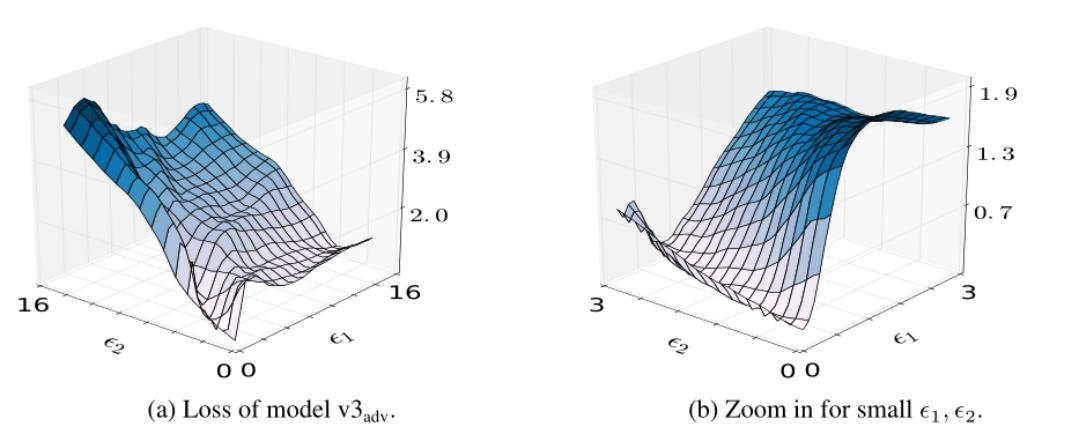
\includegraphics[width=0.8\textwidth]{fig.png}
    \caption{单步扰动攻击中存在的梯度掩盖现象}
    \label{fig:ss}
\end{figure}


如图 \ref{fig:ss} 所示,模型在该数据点处具有较高的非线性特性, 且产生梯度掩盖现象:对于未经过对抗训练的模型产生的扰动,将产生与 G' 同向的攻击, 而该模型本身的梯度方向 G 仅会到达一个局部最优。这表明,即使经过了对抗训练,模型对于其他模型转移而来的扰动攻击依然脆弱。 结论:传统的对抗训练和攻击手段的效果会因梯度掩盖而大大下降。受此启发,在扰动攻击中加入随机的分量 R 将有可能绕过梯度掩盖而产生较好效果。

\section{实验三 \; 引入随机分量的扰动攻击}
针对传统的扰动攻击的局限性,本文提出了具有随机性的扰动攻击方法,并通过实验三进行验证。其中,采用ImgNet1000数据集,对 InceptionV4, V3, V3adv, V2, V2adv 在不同种类的白盒扰动攻击下的 top1 及 top5 错误率(即攻击成功率) 进行测试。


\begin{table}[htpb]
\centering
\begin{tabular}{llllllllllll}
                    & v4            & v3            & v3adv         & IRv2          & IRv2adv       &  & v4            & v3            & v3adv         & IRv2          & IRv2adv       \\ \cline{2-6} \cline{8-12} 
   \textbf{Step-LL}    &    \pmb{60.2} & 60.9          & 26.6          & 50.7          & 21.4          &  & 31.0          & 42.7          & 9.0           & 24.0          & 5.8           \\
   \textbf{R+Step-LL}  & 70.5          & 80.0          &    \pmb{64.8} & 56.3          & 37.5          &  & 42.8          & 57.1          &    \textbf{37.1} & 29.3          & 15.0          \\
   \textbf{Iter-LL(2)} &    \pmb{78.5} &    \pmb{86.3} & 58.3          &    \pmb{69.9} &    \pmb{41.6} &  &    \pmb{56.2} &    \pmb{70.2} & 29.6          &    \pmb{45.4} &    \pmb{16.5} \\ \cline{2-6} \cline{8-12} 
                    & \multicolumn{5}{c}{Top1}                                                      &  & \multicolumn{5}{c}{Top5}                                                     
\end{tabular}
\caption{模型在白盒扰动攻击下的错误率实验结果}
\label{tab:table1}
\end{table}


实验结果如表 \ref{tab:table1} 所示,其中 Step-LL 为一种基础扰动攻击,R+Step-LL 为本文提出的随机性扰动攻击的一种形式,Iter-LL(2) 为进行两步迭代的 Step-LL 攻击。可见 R+Step-LL 攻击的效果相较于 Step-LL 在 top1 攻击成功率上有了 10$\%$ 左右的提升,在  top5 的攻击成功率上有 5$\%$ 左右的提升。结果表明,在 Step-LL 中引入随机分量 R 的攻击较不引入随机分量的攻击效果提升显著。在进 行过对抗训练的模型上,R-Step-LL 的攻击效果甚至可能优于进行 2 次迭代的 Iter-LL 攻击。


\section{实验四 \; 对抗攻击转移性证明}

实验四是针对“对抗攻击具有转移性”这一结论的证明性实验。其中,采用 ImgNet1000 数据集,将基于不同模型产生扰动攻击的样本,转移为其他模型的输入,测试攻击成功率。


\begin{table}[htbp]
\centering
\begin{tabular}{llllllllllll}
\multicolumn{6}{c}{Source}                                                        & \multicolumn{6}{c}{Source}                                                      \\
\textbf{Target} & v4            & v3            & v3adv & IRv2          & IRv2adv &\textbf{Target}  & v4      & v3            & v3adv & IRv2          & IRv2adv       \\ \hline
v4              &    \pmb{60.2} & 39.2          & 31.1  & 36.6          & 30.9    & v4      &    \pmb{31.0} & 14.9          & 10.2  & 13.6          & 9.9           \\
v3              & 43.8          &    \pmb{69.6} & 36.4  & 42.1          & 35.1    & v3      & 18.7          &    \pmb{42.7} & 13.0  & 17.8          & 12.8          \\
v3adv           &    \pmb{36.3} & 35.6          & 26.6  & 35.2          & 35.9    & v3adv   & 13.6          & 13.5          & 9.0   & 13.0          &    \pmb{14.5} \\
IRv2            & 38.0          & 38.0          & 30.8  &    \pmb{50.7} & 31.9    & IRv2    & 14.1          & 14.8          & 9.9   &    \pmb{24.0} & 10.6          \\
IRv2adv         &    \pmb{31.0} & 30.3          & 25.7  & 30.6          & 21.4    & IRv2adv & 10.3          &    \pmb{10.5} & 7.7   & 10.4          & 5.8           \\ \hline
\multicolumn{6}{c}{Top1}                                                          & \multicolumn{6}{c}{Top5}                                                       
\end{tabular}
\caption{不同模型相互扰动攻击实验结果}
\label{tab:table2}
\end{table}


实验结果如表 \ref{tab:table2} 所示,对角线上的结果为基于模型自己的扰动攻击的攻击成功率,每行的最大值直觉上应该出现在对角线上,但实验结果不然。如基于v3模型产生的扰动攻击将最有可能成功攻击 v3adv 模型(36.3$\%$)及 IRv2adv 模型(31.0$\%$)。该实验证明了扰动攻击的转移性。表明对于模型的鲁棒性测试需要同时进行黑盒和白盒攻击。 其中存在一个现象:在进行过对抗训练的模型(adv)上产生的扰动攻击在未进行过对抗 训练的模型上效果不佳,从侧面证明:对抗训练会导致模型的线性特性下降,基于这样的 模型产生的扰动攻击会因受到梯度掩盖的影响而效果不佳。



\section{实验五 \; 联合对抗训练}
本文针对扰动攻击在不同模型间可以转移的特性,提出联合对抗训练的方法。实验五是对联合对抗训练的效果进行检验的实验,其中,采用 ImgNet1000 数据集,模型如表 \ref{tab:table3}所示。


\begin{table}[htbp]
\centering
\begin{tabular}{ccc}
\textbf{Trained Model}   & \textbf{Pre-trained Model}             & \textbf{Holdout Models} \\ \hline
Inception v3(v3adv-ens3) & Inception v3, ResNet v2(50)            & Inception v4            \\
Inception v3(v3adv-ens4) & Inception v3, ResNet v2(50), IncRes v2 & ResNet v1(50)           \\
IncRes v2(IRV2adv-ens)   & Inception v3, IncRes v2                & ResNet v2(101)          \\ \hline
\end{tabular}
\caption{联合对抗训练的模型}
\label{tab:table3}
\end{table}


以训练 InceptionV3 为例,训练过程中将基于预训练好的InceptionV3,ResNetV2(50),InceptionV4模型产生扰动攻击进行一定的转化,作为InceptionV3进行对抗训练的样本进行训练。此后横向比较不同模型对于不同类型的攻击的错误率。


\begin{table}[htbp]
\centering
\begin{tabular}{ccccccc}
               & \multicolumn{3}{c}{\textbf{Top1}}                          & \multicolumn{3}{c}{\textbf{Top5}}                          \\ \cline{2-7} 
\textbf{Model} & \textbf{Clean} & \textbf{Step-LL} & \textbf{Max.Black-Box} & \textbf{Clean} & \textbf{Step-LL} & \textbf{Max.Black-Box} \\ \hline
v3             & \textbf{22.0}  & 69.6             & 51.2                   & \textbf{6.1}   & 42.7             & 24.5                   \\
v3adv          & \textbf{22.0}  & \textbf{26.6}    & 40.8                   & \textbf{6.1}   & \textbf{9.0}     & 17.4                   \\
v3adv-ens3     & 23.6           & 30.0             & \textbf{34.0}          & 7.6            & \textbf{10.1}    & \textbf{11.2}          \\
v3adv-ens4     & 24.2           & 43.3             & \textbf{33.4}          & 7.8            & 19.4             & \textbf{10.7}          \\ \hline
IRv2           & \textbf{19.6}  & 50.7             & 44.4                   & \textbf{4.8}   & 24.0             & 17.8                   \\
IRv2adv        & \textbf{19.8}  & \textbf{21.4}    & 34.5                   & \textbf{4.9}   & \textbf{5.8}     & 11.7                   \\
IRv2adv-ens    & \textbf{20.2}  & 26.0             & 27.0                   & 5.1            & 7.6              & \textbf{7.9}           \\ \hline
\end{tabular}
\caption{不同模型对于不同类型的攻击的 错误率横向对比实验结果}
\label{tab:table4}
\end{table}

联合对抗训练的效果如表 \ref{tab:table4} 所示,进行传统对抗训练的模型被标记为  adv,进行本文提出的联合对抗训练的模型被标记为  adv-ens。实验结果表明,进行联合对抗训练的模型虽然在应对白盒攻击的稳健性上略低 于传统对抗训练,但对于黑盒攻击,模型的稳健性有明显提升。该实验证明了本文提出的训练方法的优越性。